%%%%%%%%%%%%%%%%%%%%%%%%%%
\chapter{Polyphonic Sound Event Detection}
\section{Sound Event Detection in Real Life Audio}

\section{Introduction}
\label{sec:intro}


Automatic sound event detection (SED), also known as acoustic event detection, is nowadays considered as one of the most important topics in the field of computational auditory scene analysis (CASA). Thanks to works like Bregman's ``Auditory Scene Analysis: The Perceptual Organization of Sound''~\cite{bregman1994auditory}, we can trace back the birth of this field to 1994, when the field of auditory scene analysis (ASA) was introduced in order to model humans' sound perception. Following this work, many other contributions were written aiming to describe how artificial systems can be designed in order to perceive sounds similarly to as humans do; most of these works will be later collected in Divenyi's book~\cite{divenyi2004speech} in 2004.

SED is defined as the task of analysing a continuous audio signal in order to extract a description of the sound events occurring in the audio stream. This description is commonly expressed as a label that marks the start, the ending, and the nature of the occurred sound (\emph{e.g.,}\ children crying, cutlery, glass jingling). In particular, in multi-label SED it is assumed that more than one event can be active (and should be detected) at a time, therefore foreseeing the overlapping of two or more of these labels. This problem is addressable as a ``mixture problem'' and it is usually not trivial to solve mainly due to the superimposition of different event energies in the audio spectra.

Labels extracted with a SED system usually allow us to achieve a better insight of the considered acoustic scenario, for example they can be used as mid-level representation useful for other CASA research areas. In~\cite{chu2009environmental, heittola2010audio}, for example, authors make use of SED for designing audio context recognition systems, while in~\cite{shah2012lifelogging} and~\cite{wichern2010segmentation} SED is exploited for automatic tagging and audio segmentation respectively. Moreover, SED also found many direct applications in a variety of scenarios, some examples being context-based indexing and retrieval in multimedia databases~\cite{xu2008audio}, unobtrusive health monitoring~\cite{peng2009healthcare}, and audio-based surveillance~\cite{harma2005automatic, crocco2014surveillance, Principi2016a}.

As we can notice from~\cite{heittola2010audio, peng2009healthcare}, hidden Markov models (HMMs) have been widely used in the literature with the purpose of modelling acoustic events in a SED system, usually in terms of a Gaussian mixture model (GMM). In recent years, new approaches to SED have been proposed, marking a distinct trend towards the use of artificial neural networks (ANNs)-based systems. An interesting comparison between computational costs of different systems is carried out in~\cite{sigtia2016automatic} highlighting that ANNs are able to achieve top performance at the cost of being the most computationally expensive approach. A brilliant example of such performance is given in~\cite{hershey2016cnn}, where different ANNs are trained on a big video dataset and then used for different scopes, among which also SED. For a wider overview of the most recent and powerful SED techniques the reader can refer to the comprehensive analysis carried out by Sharan \emph{et al.}\ in~\cite{sharan2016overview}.

In occasion of the Detection and Classification of Acoustic Scenes and Events (DCASE) 2016 challenge, many novel systems featuring recurrent neural networks (RNNs) and multilayer perceptrons (MLPs) have been proposed, even though only one of them~\cite{adavanne2016sound} managed to outperform the baseline system (based on a GMM) thus reaching the first rank in the challenge third task. In the authors' opinion, this proves that there is still a lot of space for research in approaching SED with ANNs, therefore we here propose a system which relies on a voice activity detection (VAD) algorithm for the detection of acoustic events which are then classified by an ANN. During our experiments we compare different well-established audio representation, \emph{i.e.,}\ log-mel energies and mel-frequency cepstral coefficients (MFCCs), extracted in both monaural and binaural configuration. Moreover, we will evaluate two VAD algorithms (\emph{i.e.,}\ adaptive energy (AE) and Sohn's VAD), as well as two different ANN architectures for classification, \emph{i.e.,}\ MLPs and RNNs. Our aim is therefore to give a novel contribution by presenting a robust system capable to improve the results obtained by participants to the DCASE 2016 challenge.

In Section~\ref{sec:prop_meth} we present the method proposed for the SED task, we therefore describe the feature extraction processes, the proposed neural architectures and the VAD algorithms we tested. In Section~\ref{sec:eval} we describe the dataset and the metrics used to evaluate our system, and, together with our experimental setup, we report our main results. Finally, in Section~\ref{sec:conclusions} we draw our conclusions and highlight some possibilities for future development of new SED systems.

\section{Proposed method}
\label{sec:prop_meth}

As we can see from Figure~\ref{fig:system_scheme} it is possible to divide the system functioning into two phases: training and testing. During training we do not need to use any algorithm for event detection, since onset and offset instants are already provided in the ground truth, therefore we can simply train an ANN to recognise the different events. At test time, on the other hand, onset and offset instants are not given, therefore we firstly make use of a VAD algorithm for determining them, and secondly we feed the corresponding audio sequences to the ANN classifier.

\begin{figure}[t]
	\centering
	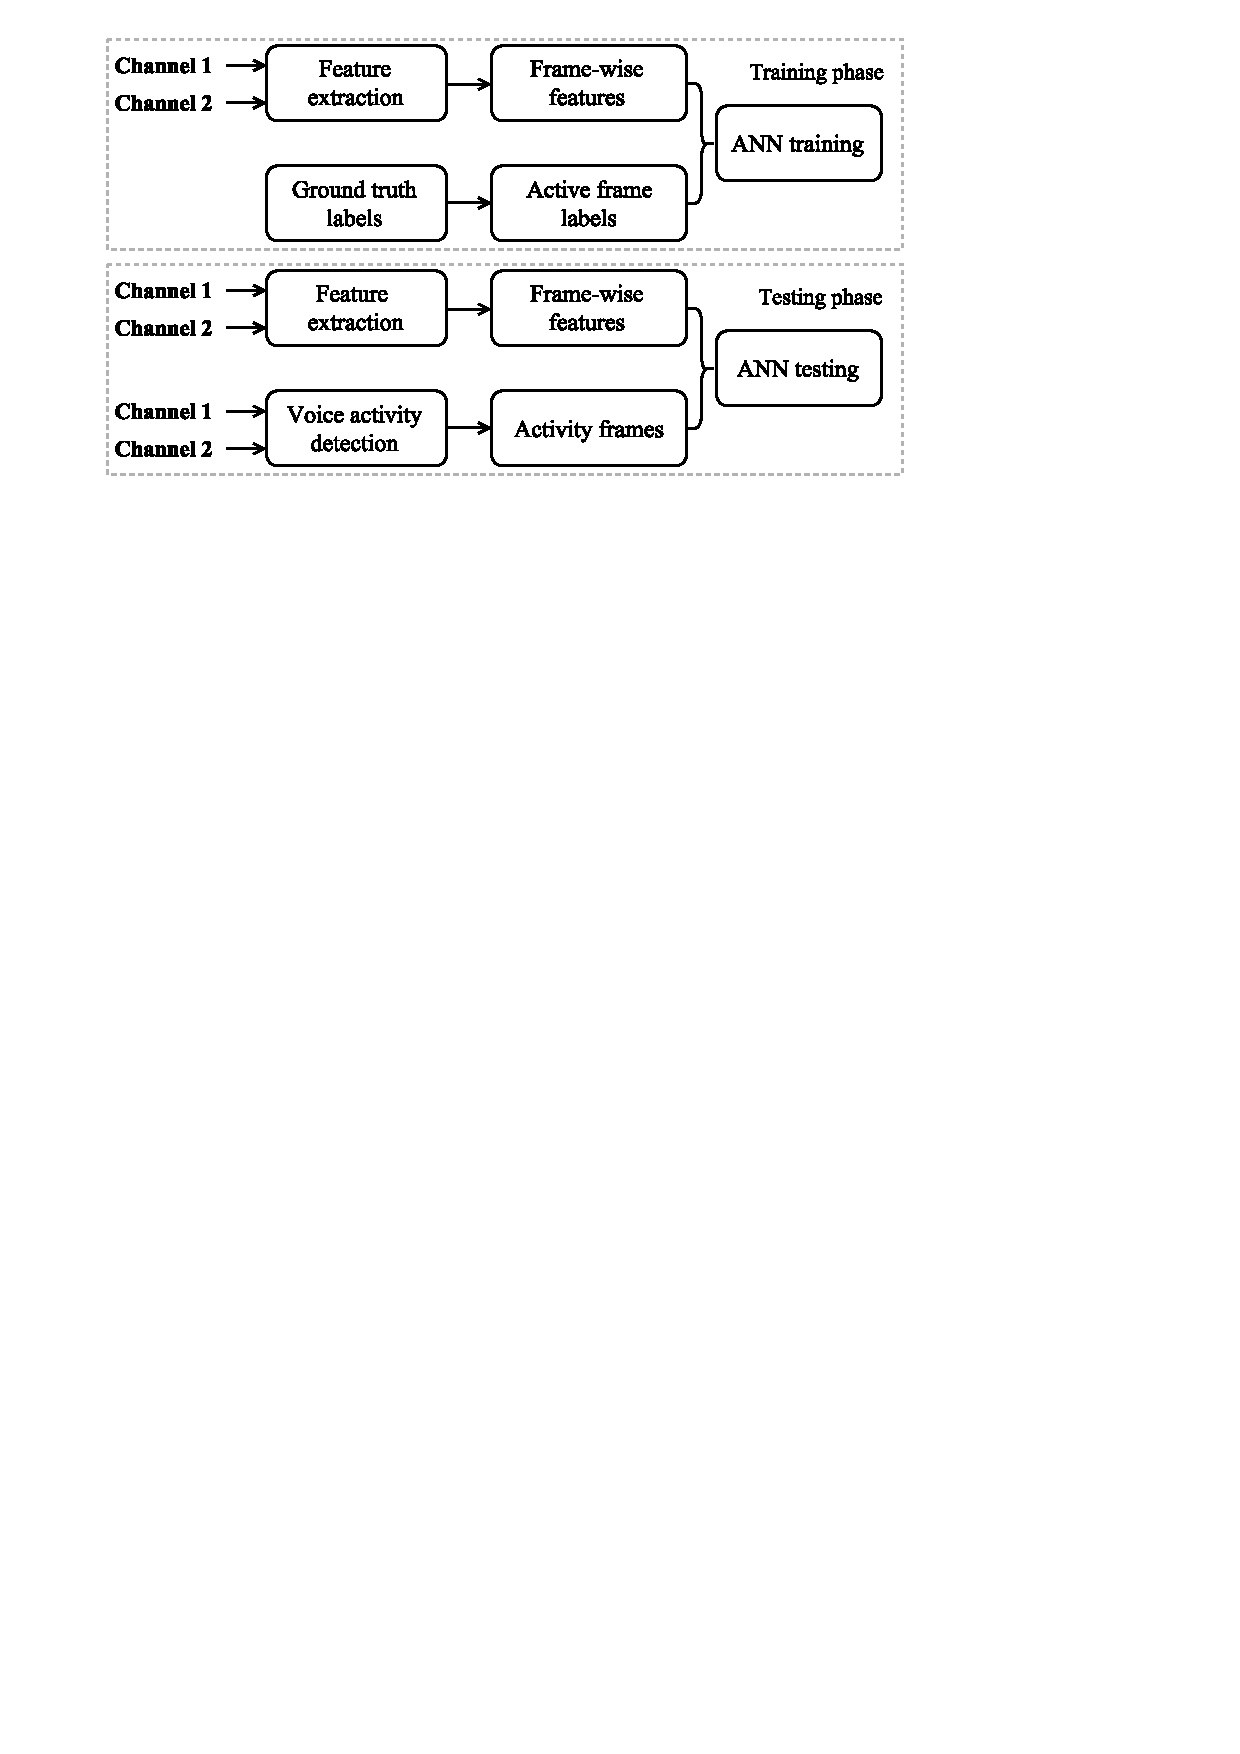
\includegraphics[width=0.47\textwidth]{figures/system_scheme.pdf}
	\caption{Block diagram of training and testing phases. At test time a VAD algorithm is used to determine onset and offset instants of the detected events.}
	\label{fig:system_scheme}
\end{figure}

\subsection{Feature representations}

In order to perform the SED task with ANNs, a set of one or more audio representations is typically extracted from the raw audio signal, that is the \emph{feature set}. Aiming to evaluate the impact of binaural information on the classification performance, we will, in the first instance, distinguish the proposed sets between monaural and binaural feature sets. We highlight that, for all the extracted feature sets, a frame-wise short-time Fourier transform (STFT) is firstly applied to the audio signal on frame windows of 40 ms with 50\% overlap. Moreover, all feature extraction processes described hereafter have been performed with openSMILE~\cite{eyben2013recent}, a license-free software package developed by the Technical University of Munich.

The first monaural set is known as log-mel spectrogram. In this case a down-mixing of the two audio channels is required before calculating the STFT coefficients. After the STFT coefficients are extracted, we apply a mel conversion of the frequency scale with a 26-bands mel-scale filter bank and compute the logarithm of all the energies so obtained. To complete the set, we also extract the first order delta coefficients operating on a context window of 10 frames. Given the log-mel coefficients and their respective deltas, this first set is composed of 52 coefficients for each frame.

The second monaural set is composed of another set of widely used features, that is mel-frequency cepstral coefficients (MFCCs). Starting from the same STFT coefficients previously obtained, we now compute the log-mel spectrogram with a 40-bands mel-scale filter bank. Then, we apply a 20-points discrete cosine transform (DCT) to each energy vector and, after excluding the 0\textsuperscript{th} order coefficient, we obtain a feature vector of 20 MFCCs. In order to complete the set, we also calculate the first and second order delta coefficients, therefore obtaining a 60-coefficients feature vector.

For the two binaural sets we decided to extract the log-mel (or the MFCC) features not only from the average of the two channels, but also from their difference and the two separate channels; this gives us a total of four channels. We decided to do so because, for example, if an important event is predominant in only one of the two channels, averaging them could lower the signal-to-noise ratio, thus increasing the system failure probability. For the first binaural set we extract the log-mel coefficients as for the first monaural set, but, given the presence of four channels, we now have a total of 108 coefficients for each frame. In order to avoid an excessive feature vector dimension, in this set we decide to avoid using the first and second order delta coefficients. Similarly, the second binaural set is obtained by extracting 20 MFCCs for each channel; since again we avoid using the delta coefficients, this leads us to a total of 80 coefficients for each frame. 

\subsection{Neural networks}

In this work two different ANNs architectures are tested for the SED problem, \emph{i.e.,}\ MLPs and RNNs. Asides from single layer perceptrons, MLPs can be considered to be the most simple (yet very effective) form of ANN. A MLP is composed of an ensemble of many nonlinear computational units (called neurons) organized in a layered structures. Thanks to the full connectedness of neurons between two sequent layers, each of them is likely trained to recognize a particular pattern occurring in a specific input position, therefore making the MLP able to build high level feature representations in deeper layers. 

RNNs, on the other hand, are a particular neural architecture designed to make use of the information obtained from prior network states, therefore giving the network the capability to ``remember'' past context information. This feature is obtained by adding a set of recursive connections going from and to each hidden neuron. Due this characteristic, the output is now computed only after a batch of input frames are forwarded into the network so that the final decision will rely on the correlation between different adjacent frames.

The first layer of all proposed ANNs consists of a set of nodes to which the audio representation (taken on a frame scale) is applied, with the number of nodes varying from 52 to 108, depending on the chosen feature representation. The input is then propagated to the following three hidden layers, composed of 512 tanh neurons each for MLPs and 54 rectifier neurons for RNNs.  Finally, the last layer of our networks is designed to output the class associated by the network with the given input. To do so, this layer is composed of a number of softmax neurons equal to the number of possible classes, \emph{i.e.,} 11 if we are dealing with a ``home'' scenario, and 7 in case of a ``residential area'' (see Tab.~\ref{tab:classes}). We highlight that, in case of MLPs, we obtain one label for each frame, whereas RNNs are able to output one label also for a batch of sequent frames.

The standard algorithm used for training the proposed MLPs is the backpropagation (BP) algorithm, whereas for RNNs the ``BP through time'' is used. After a first feed-forward phase, in which a batch of input is propagated through the networks, these algorithms exploit the derivative ``chain rule'' to back-propagate the error computed at the output layer and sequentially update all neuron weights~\cite{rojas2013neural}.

\subsection{Sound event detection and classification}

At test time we want the system to detect and correctly classify as many acoustic events as possible occurring in raw audio files of 30 seconds. Since no onset nor offset instants are given, we decide to use VAD algorithms in order to detect these instants. With this intent, two different VAD algorithms have been tested, \emph{i.e.,}\ AE, and Sohn's VAD. 

The AE approach makes use of two energy thresholds in order to determine the starting and ending point of an event-active audio sequence, \emph{i.e.,}\ the ``mean plus variance'' (MPV) and the ``mean minus variance'' (MMV) thresholds. These thresholds are firstly calculated over all the training dataset and then used to extract information about events activity: whenever a frame's energy exceeds the MPV threshold an onset event is triggered, then the event detection remains positive until the energy content drops below the MMV threshold. 

Sohn's VAD~\cite{sohn1999statistical}, on the other hand, is a method based on a statistical modelling of the audio in the time-frequency domain, with the model parameters being estimated with a maximum likelihood (ML) method. With this technique, the decision regarding the event's activity is devolved to a comparison between the averaged log-likelihood ratio (containing the a-priori and a-posteriori signal-to-noise ratios) and a fixed threshold $\eta \in (0,1)$. 

Whenever an audio file is processed by one of the two VAD algorithms we are able to extract the starting and ending instants between which an audio event has (supposedly) occurred. Hence, we can feed the network with the feature representation of the corresponding frames and finally obtain the event classification. We remind that, in case of MLPs, we obtain one label for each frame, whereas RNNs are able to output only one label for the whole frame batch. Due to this, we need to average all MLP outputs so to obtain the event's acoustic label, while RNN's outputs will need no further processing.

\section{Experiments}
\label{sec:eval}

\subsection{Datasets and metrics}

The data we use during our experiments consist of two datasets provided for the third task (SED in real life audio) of the DCASE 2016 challenge~\cite{mesaros2016tut}. The former dataset, called \emph{development dataset}, was at first provided in order to make all challengers able to compare their development results, while the latter, the \emph{evaluation dataset}, was used for the final evaluation of the submitted systems, so its ground truth was made public only a few weeks after the end of the challenge. Both datasets contains recordings of 3-5 minutes divided into two different acoustic scenarios: ``home'' and ``residential area''. Specific classes for each scenario are reported in Table~\ref{tab:classes}. 

%\begin{table}
%\caption{Classes for the ``home'' and ``residential area'' scenarios provided for the SED in real life audio task of the DCASE 2016 challenge.}
%\label{tab:classes}
%\centering
%\begin{tabular}{l l | l l}\toprule
%\multicolumn{2}{c}{\emph{Home}} & \multicolumn{2}{c}{\emph{Residential area}}\\
%\midrule
%rustling & glass jingling & banging & wind blowing\\
%snapping & object impact & bird singing\\
%cupboard & people walking & car passing by\\
%cutlery & washing dishes & children shouting\\
%dishes & water tap running & people walking  \\
%drawer & & people speaking \\
%\bottomrule
%\end{tabular}
%\end{table}

\begin{table}
	\caption{Classes and their occurrences for the ``home'' and ``residential area'' scenarios for the SED in real life audio task of the DCASE 2016 challenge.}
	\label{tab:classes}
	\centering
	\begin{tabular}{l c l c}\toprule
		\emph{Home} & \emph{Occurrences} & \emph{Residential area} & \emph{Occurrences}\\
		\midrule
		rustling & 60 & banging & 23\\
		snapping & 57 & bird singing & 271\\
		cupboard & 40 & car passing by & 108\\
		cutlery & 76 & children shouting & 31\\
		dishes & 151 & people walking & 52 \\
		drawer & 51 & people speaking & 44\\
		glass jingling & 36 & wind blowing & 30\\
		object impact & 250\\
		people walking & 54\\
		washing dishes & 84\\
		water tap running & 47\\
		\bottomrule
	\end{tabular}
\end{table}

The development dataset consists of 10 recordings for the ``home'' scenario, and 12 for the ``residential area'', and for both a four-folds cross-validation data splitting is provided by the organizers of the challenge. While creating the cross-validation folds, the challenge organizers imposed the only condition that the test subset does not contain classes unavailable in training subset, therefore the class distribution between the test subsets is not assumed to be uniform.

The evaluation dataset contains 5 recordings for both the ``home'' and the ``residential area'' scenarios each. For this dataset no cross-validation is performed, so it is possible to train only one system with all the development dataset (including files previously meant for testing purpose) and then test it with the evaluation files.

Scores used to evaluate all systems are the well known F1 and error rate (ER) scores, which are used to evaluate the system over segments of one second. Following the notation introduced in~\cite{mesaros2016tut}, for the evaluation purpose an event can be a: true positive (TP), if both the system and the ground truth indicate it as active; a false positive (FP), if the system indicates it as active, but it is not present in the ground truth; a false negative (FN), if the system does not detect it, but it is active in the ground truth. With this notation it is possible to define the precision (P), the recall (R), and the F1 score of the system as:
\begin{equation}
\text{P}=\frac{\text{TP}}{\text{TP}+\text{FP}}, \quad \text{R}=\frac{\text{TP}}{\text{TP}+\text{FN}}, \quad \text{F1}=\frac{2 \cdot \text{P} \cdot \text{R}}{\text{TP}+\text{FN}}.
\end{equation}

Concerning the ER, we must divide all possible errors into three categories: substitutions (S), insertions (I), and deletions (D). A substitution occurs when the system correctly detects an event but gives it the wrong label; moreover, we consider insertions all those FPs which are not substitutions, whereas we call deletions all those FNs which are not substitutions. According to this notation we define the ER as:
\begin{equation}
\text{ER} = \frac{\sum_{k=1}^{K} \text{S}(k) + \sum_{k=1}^{K} \text{D}(k) + \sum_{k=1}^{K} \text{I}(k)}{\sum_{k=1}^{K} \text{N}(k)},
\end{equation}
where $\text{N}(k)$ is the number of active events in the ground truth, and $k$ is the segment's index. Finally we highlight that, in obtaining the final score for the development dataset, we average the four per-fold scores as described in~\cite{mesaros2016tut}.

\subsection{Experimental setup}

Concerning the network training, we initialize all weights according to a normal distribution with zero mean and 0.1 variance. We then train the networks following the adam~\cite{kingma2014adam} method for stochastic optimization, for which we keep the default hyper-parameter configuration.

In order to prevent overfitting, for each fold we check the network performance on the respective fold's test set after each training epoch. If no improvement on this set is encountered for 60 consecutive epochs, the training is forced to an early stop. By doing so we are able to fine-tune the network hyper-parameters and obtain the architectures proposed in Section~\ref{sec:prop_meth}. 

After this phase we perform experiments on the evaluation data, for which we use the whole development training and test sets as training and validation data respectively. Then, at test time, we evaluate the system on the secret challenge data.

\subsection{Development results}

As introduced in Section~\ref{sec:prop_meth}, during our experiments we tested and compared different neural architectures, VAD algorithms, and feature representations. In Table~\ref{tab:dev_results_sohn} we report the results obtained with Sohn's VAD for 16 different system configurations, whereas in Table~\ref{tab:dev_results_ae} the same classifier and feature configurations are analysed in conjunction with AE VAD.

Table~\ref{tab:dev_results_sohn} highlights that the use of binaural audio features always enhances the system's performance in terms of both F1 and ER scores. Moreover, we can also notice that MLPs generally perform better than RNNs, in particular according to F1 scores, where no RNN manages to achieve more than 34.4\% F1 score. Finally, we report that the best system's configuration featuring Sohn's VAD is a MLP trained with binaural MFCC features, with a VAD threshold equal to 0.70. This system manages to reach 0.88 ER and 39.8\% F1 score, both averaged on the four folds.

\begin{table}
	\caption{Comparison of Scores obtained on the development dataset using different Features, Classifiers and Sohn's VAD Thresholds ($\eta$). Scores are Averaged among the four Cross-Validation Folds.}
	\label{tab:dev_results_sohn}
	\centering
	\begin{tabular}{l c c c c}\toprule
		\emph{Features} & \emph{$\eta$} & \emph{Classifier} & \emph{ER} & \emph{F1} (\%)\\
		\midrule
		Monaural log-mel & 0.98 & MLP & 0.93 & 34.6\\
		Binaural log-mel & 0.98 & MLP & 0.89 & 38.6\\
		\midrule
		Monaural log-mel & 0.70 & MLP & 0.90 & 35.4\\
		Binaural log-mel & 0.70 & MLP & 0.89 & 39.4\\
		\midrule
		Monaural MFCC & 0.98 & MLP & 0.92 & 35.7\\
		Binaural MFCC & 0.98 & MLP & 0.88 & 39.6\\
		\midrule
		Monaural MFCC & 0.70 & MLP & 0.91 & 36.2\\
		\textbf{Binaural MFCC} & \textbf{0.70} & \textbf{MLP} & \textbf{0.88} & \textbf{39.8}\\
		\midrule
		Monaural log-mel & 0.98 & RNN & 0.91 & 29.6\\
		Binaural log-mel & 0.98 & RNN & 0.88 & 35.6\\
		\midrule
		Monaural log-mel & 0.70 & RNN & 0.95 & 28.2\\
		Binaural log-mel & 0.70 & RNN & 0.88 & 34.4\\
		\midrule
		Monaural MFCC & 0.98 & RNN & 0.98 & 30.5\\
		Binaural MFCC & 0.98 & RNN & 0.88 & 34.1\\
		\midrule
		Monaural MFCC & 0.70 & RNN & 0.91 & 31.2\\
		Binaural MFCC & 0.70 & RNN & 0.88 & 31.0\\
		\bottomrule
	\end{tabular}
\end{table}

Table~\ref{tab:dev_results_ae} mostly confirms what emerged from the analysis of the previous table. Also with adaptive evergy VAD, the use of binaural features always improves the classification accuracy, even if differences are now less marked, with the highest improvement in F1 scores being +2\%. Moreover, it is interesting to notice that the difference between MLPs and RNNs accuracies is now reduced, maybe highlighting that the difference between their classification power thins if a better VAD algorithm leads to a better event detection. The best performing system featuring AE VAD is again a MLP which, with binaural log-mel features, manages to reach 0.78 ER and 43.1\% F1 scores, averaged on the four folds as for the previous results.

\begin{table}
	\caption{Comparison of Scores obtained on the development dataset using different Features, Classifiers and AE VAD. Scores are Averaged among the four Cross-Validation Folds.}
	\label{tab:dev_results_ae}
	\centering
	\begin{tabular}{l c c c}\toprule
		\emph{Features} & \emph{Classifier} & \emph{ER} & \emph{F1} (\%)\\
		\midrule
		Monaural log-mel & MLP & 0.78 & 41.2\\
		\textbf{Binaural log-mel} & \textbf{MLP} & \textbf{0.78} & \textbf{43.1}\\
		\midrule
		Monaural MFCC & MLP & 0.81 & 40.1\\
		Binaural MFCC & MLP & 0.82 & 42.1\\
		\midrule
		Monaural log-mel & RNN & 0.85 & 41.2\\
		Binaural log-mel & RNN & 0.82 & 43.1\\
		\midrule
		Monaural MFCC & RNN & 0.92 & 40.7\\
		Binaural MFCC & RNN & 0.89 & 41.0\\
		\bottomrule
	\end{tabular}
\end{table}

\subsection{Evaluation results}

\begin{table}
	\caption{Comparison of Scores obtained on the Evaluation Dataset using different Features, Classifiers and VAD Algorithms.}
	\label{tab:eval_results}
	\centering
	\begin{tabular}{l c c c c}\toprule
		\emph{Features} & \emph{VAD} & \emph{Classifier} & \emph{ER} & \emph{F1} (\%)\\
		\midrule
		Monaural log-mel & Sohn ($\eta=0.70$) & MLP & 0.80 & 40.2\\
		Binaural log-mel & Sohn ($\eta=0.70$) & MLP & 0.78 & 46.5\\
		\midrule
		Monaural MFCC & AE & MLP & 0.79 & 45.1\\
		\textbf{Binaural MFCC} & \textbf{AE} & \textbf{MLP} & \textbf{0.78} & \textbf{48.1}\\
		\midrule
		Monaural MFCC & AE & RNN & 0.82 & 41.0\\
		\bottomrule
	\end{tabular}
\end{table}

\begin{table}
	\caption{Comparison Between the proposed System and the three (out of 17) best performing DCASE 2016 Systems proposed for SED in real life audio.}
	\label{tab:challenge_results}
	\centering
	\begin{tabular}{l c c c c}\toprule
		\emph{Features} & \emph{VAD} & \emph{Classifier} & \emph{ER} & \emph{F1} (\%)\\
		\midrule
		\textbf{Binaural log-mel} & \textbf{AE} & \textbf{MLP} & \textbf{0.79} & \textbf{48.1}\\
		\midrule
		Binaural mel energy & - & RNN~\cite{adavanne2016sound} & 0.81 & 47.8\\
		Binaural mel energy & - & GMM~\cite{mesaros2016tut} & 0.88 & 23.7\\
		Binaural mel energy + TDOA & - & RNN~\cite{adavanne2016sound} & 0.89 & 34.3\\
		\bottomrule
	\end{tabular}
\end{table}

In Table~\ref{tab:eval_results} we report the main results for the most promising system configurations tested on the evaluation dataset. As we can see, scores tend to be higher than the ones obtained on the development dataset, especially for MLPs, highlighting the benefit introduced by the addition in the training set of those files previously used for testing. The expansion of the training set can be viewed as the expansion of the ``knowledge'' from which the network can learn at training time, therefore, when this happens, it is expectable to reach a better generalization performance. This behaviour is confirmed, the best performing configuration manages to achieve a 0.79 ER and 48.1\% F1 scores, and it consists of a MLP classifier trained on binaural MFCC features.

Table~\ref{tab:challenge_results} compares our best system to the three best performing ones proposed for the third task of the DCASE 2016 challenge. The first and the third ranks were achieved by Adavanne \emph{et al.}, which made use of RNN-LSTM architectures trained on spatial and harmonic features~\cite{adavanne2016sound} extracted from the two binaural channels. On the other hand, the second best system is the baseline proposed in~\cite{mesaros2016tut}, based on a GMM modelling of each acoustic event, plus one for the absence of sound events, which was trained with the non-labelled frame's features (MFCCs and their delta/delta-deltas were used). As we can see from the table, the proposed system manages to improve the F1 score by 0.3\% while reducing the error rate by 0.02.

\section{Conclusions and future work}
\label{sec:conclusions}

In this paper we proposed and evaluated a system for SED in real life audio. We compared different audio features, extracted in both monaural and binaural configurations, with which we trained different neural network classifiers. Moreover, we tested two different VAD algorithms for detecting sound activities to be classified by the proposed networks at test time. The proposed best performing system achieves an improvement on the winner of the third task in the DCASE 2016 challenge, thus highlighting the competitiveness of the proposed approach. Finally, given the improvement carried by the use of binaural features, we believe that future work should address the development of a binaural algorithm using one or more networks for each channel and a decision function for a decision fusion stage.